\ifdefined\included
\else
\documentclass[a4paper,11pt,twoside]{StyleThese}
\usepackage{amsmath,amssymb, amsthm}             % AMS Math
\usepackage[T1]{fontenc}
\usepackage[utf8x]{inputenc}
\usepackage{babel}
\usepackage{datetime}

\usepackage{silence}

\WarningFilter{minitoc(hints)}{W0023}
\WarningFilter{minitoc(hints)}{W0028}
\WarningFilter{minitoc(hints)}{W0030}

\usepackage{lmodern}
\usepackage{tabularx}
%\usepackage{tabular}
\usepackage{multirow}
\usepackage{xspace}

\usepackage{hhline}
\usepackage[left=1.5in,right=1.3in,top=1.1in,bottom=1.1in,includefoot,includehead,headheight=13.6pt]{geometry}
\renewcommand{\baselinestretch}{1.05}

% Table of contents for each chapter

\usepackage[nottoc, notlof, notlot]{tocbibind}
\usepackage{minitoc}
\setcounter{minitocdepth}{2}
\mtcindent=15pt
% Use \minitoc where to put a table of contents

\usepackage{aecompl}

% Glossary / list of abbreviations

\usepackage[intoc]{nomencl}
\iftoggle{ThesisInEnglish}{%
\renewcommand{\nomname}{Glossary}
}{ %
\renewcommand{\nomname}{Liste des Abréviations}
}

\usepackage{etoolbox}
\renewcommand\nomgroup[1]{%
  \item[\bfseries
  \ifstrequal{#1}{A}{Number Sets}{%
  \ifstrequal{#1}{G}{Agents Beliefs and Action Models}{%
  \ifstrequal{#1}{N}{Navigation}{%
  \ifstrequal{#1}{O}{Ontology}{%
  \ifstrequal{#1}{R}{Referring Expression Generation}{%
  \ifstrequal{#1}{Z}{Controllable and Uncontrollable Agents Task Planning}{}}}}}}%
]}

\makenomenclature



% My pdf code

\usepackage{ifpdf}

\ifpdf
  \usepackage[pdftex]{graphicx}
  \DeclareGraphicsExtensions{.jpg}
  \usepackage[pagebackref,hyperindex=true]{hyperref}
  \usepackage{tikz}
  \usetikzlibrary{arrows,shapes,calc}
\else
  \usepackage{graphicx}
  \DeclareGraphicsExtensions{.ps,.eps}
  \usepackage[dvipdfm,pagebackref,hyperindex=true]{hyperref}
\fi

\graphicspath{{.}{images/}}

%% nicer backref links. NOTE: The flag ThesisInEnglish is used to define the
% language in the back references. Read more about it in These.tex

\iftoggle{ThesisInEnglish}{%
\renewcommand*{\backref}[1]{}
\renewcommand*{\backrefalt}[4]{%
\ifcase #1 %
(Not cited.)%
\or
(Cited in page~#2.)%
\else
(Cited in pages~#2.)%
\fi}
\renewcommand*{\backrefsep}{, }
\renewcommand*{\backreftwosep}{ and~}
\renewcommand*{\backreflastsep}{ and~}
}{%
\renewcommand*{\backref}[1]{}
\renewcommand*{\backrefalt}[4]{%
\ifcase #1 %
(Non cité.)%
\or
(Cité en page~#2.)%
\else
(Cité en pages~#2.)%
\fi}
\renewcommand*{\backrefsep}{, }
\renewcommand*{\backreftwosep}{ et~}
\renewcommand*{\backreflastsep}{ et~}
}

% Links in pdf
\usepackage{color}
\definecolor{linkcol}{rgb}{0,0,0.4} 
\definecolor{citecol}{rgb}{0.5,0,0} 
\definecolor{linkcol}{rgb}{0,0,0} 
\definecolor{citecol}{rgb}{0,0,0}
% Change this to change the informations included in the pdf file

\hypersetup
{
bookmarksopen=true,
pdftitle="Planning For Both Robot and Human: Anticipating and Accompanying Human Decisions",
pdfauthor="Guilhem BUISAN", %auteur du document
pdfsubject="Thèse", %sujet du document
%pdftoolbar=false, %barre d'outils non visible
pdfmenubar=true, %barre de menu visible
pdfhighlight=/O, %effet d'un clic sur un lien hypertexte
colorlinks=true, %couleurs sur les liens hypertextes
pdfpagemode=None, %aucun mode de page
pdfpagelayout=SinglePage, %ouverture en simple page
pdffitwindow=true, %pages ouvertes entierement dans toute la fenetre
linkcolor=linkcol, %couleur des liens hypertextes internes
citecolor=citecol, %couleur des liens pour les citations
urlcolor=linkcol %couleur des liens pour les url
}

% definitions.
% -------------------

\setcounter{secnumdepth}{3}
\setcounter{tocdepth}{2}

% Some useful commands and shortcut for maths:  partial derivative and stuff

\newcommand{\pd}[2]{\frac{\partial #1}{\partial #2}}
\def\abs{\operatorname{abs}}
\def\argmax{\operatornamewithlimits{arg\,max}}
\def\argmin{\operatornamewithlimits{arg\,min}}
\def\diag{\operatorname{Diag}}
\newcommand{\eqRef}[1]{(\ref{#1})}

\usepackage{rotating}                    % Sideways of figures & tables
%\usepackage{bibunits}
%\usepackage[sectionbib]{chapterbib}          % Cross-reference package (Natural BiB)
%\usepackage{natbib}                  % Put References at the end of each chapter
                                         % Do not put 'sectionbib' option here.
                                         % Sectionbib option in 'natbib' will do.
\usepackage{fancyhdr}                    % Fancy Header and Footer

% \usepackage{txfonts}                     % Public Times New Roman text & math font
  
%%% Fancy Header %%%%%%%%%%%%%%%%%%%%%%%%%%%%%%%%%%%%%%%%%%%%%%%%%%%%%%%%%%%%%%%%%%
% Fancy Header Style Options

\pagestyle{fancy}                       % Sets fancy header and footer
\fancyfoot{}                            % Delete current footer settings

%\renewcommand{\chaptermark}[1]{         % Lower Case Chapter marker style
%  \markboth{\chaptername\ \thechapter.\ #1}}{}} %

%\renewcommand{\sectionmark}[1]{         % Lower case Section marker style
%  \markright{\thesection.\ #1}}         %

\fancyhead[LE,RO]{\bfseries\thepage}    % Page number (boldface) in left on even
% pages and right on odd pages
\fancyhead[RE]{\bfseries\nouppercase{\leftmark}}      % Chapter in the right on even pages
\fancyhead[LO]{\bfseries\nouppercase{\rightmark}}     % Section in the left on odd pages

\let\headruleORIG\headrule
\renewcommand{\headrule}{\color{black} \headruleORIG}
\renewcommand{\headrulewidth}{1.0pt}
\usepackage{colortbl}
\arrayrulecolor{black}

\fancypagestyle{plain}{
  \fancyhead{}
  \fancyfoot{}
  \renewcommand{\headrulewidth}{0pt}
}

%\usepackage{MyAlgorithm}
%\usepackage[noend]{MyAlgorithmic}
\usepackage{algorithm}
\usepackage[noend]{algpseudocode}
\usepackage{comment}
\usepackage[ED=EDSYS-Robo, Ets=INSA]{tlsflyleaf}
%%% Clear Header %%%%%%%%%%%%%%%%%%%%%%%%%%%%%%%%%%%%%%%%%%%%%%%%%%%%%%%%%%%%%%%%%%
% Clear Header Style on the Last Empty Odd pages
\makeatletter

\def\cleardoublepage{\clearpage\if@twoside \ifodd\c@page\else%
  \hbox{}%
  \thispagestyle{empty}%              % Empty header styles
  \newpage%
  \if@twocolumn\hbox{}\newpage\fi\fi\fi}

\makeatother
 
%%%%%%%%%%%%%%%%%%%%%%%%%%%%%%%%%%%%%%%%%%%%%%%%%%%%%%%%%%%%%%%%%%%%%%%%%%%%%%% 
% Prints your review date and 'Draft Version' (From Josullvn, CS, CMU)
\newcommand{\reviewtimetoday}[2]{\special{!userdict begin
    /bop-hook{gsave 20 710 translate 45 rotate 0.8 setgray
      /Times-Roman findfont 12 scalefont setfont 0 0   moveto (#1) show
      0 -12 moveto (#2) show grestore}def end}}
% You can turn on or off this option.
% \reviewtimetoday{\today}{Draft Version}
%%%%%%%%%%%%%%%%%%%%%%%%%%%%%%%%%%%%%%%%%%%%%%%%%%%%%%%%%%%%%%%%%%%%%%%%%%%%%%% 

\newenvironment{maxime}[1]
{
\vspace*{0cm}
\hfill
\begin{minipage}{0.5\textwidth}%
%\rule[0.5ex]{\textwidth}{0.1mm}\\%
\hrulefill $\:$ {\bf #1}\\
%\vspace*{-0.25cm}
\it 
}%
{%

\hrulefill
\vspace*{0.5cm}%
\end{minipage}
}

\let\minitocORIG\minitoc
\renewcommand{\minitoc}{\minitocORIG \vspace{1.5em}}

\usepackage{multirow}
%\usepackage{slashbox}

\newenvironment{bulletList}%
{ \begin{list}%
	{$\bullet$}%
	{\setlength{\labelwidth}{25pt}%
	 \setlength{\leftmargin}{30pt}%
	 \setlength{\itemsep}{\parsep}}}%
{ \end{list} }

\theoremstyle{definition}
\newtheorem{definition}{Definition}
\renewcommand{\epsilon}{\varepsilon}

% centered page environment

\newenvironment{vcenterpage}
{\newpage\vspace*{\fill}\thispagestyle{empty}\renewcommand{\headrulewidth}{0pt}}
{\vspace*{\fill}}

\usepackage{tablefootnote}

\theoremstyle{plain}
\newtheorem{constraint}{Constraint}[section]

\algnewcommand\algorithmicforeach{\textbf{for each}}
\algnewcommand\algorithmicin{\textbf{in}}
\algdef{S}[FOR]{ForEach}[2]{\algorithmicforeach\ #1\ \algorithmicin\ #2\ \algorithmicdo}

\usepackage{listings}
\lstdefinestyle{customPlan}{
  language=C,
  commentstyle=\itshape\color{green!25!black},
}
\usepackage{pdfpages}

\sloppy
\begin{document}
\setcounter{chapter}{0} %% Numéro du chapitre précédent ;)
\dominitoc
\faketableofcontents
\fi

\chapter{Planning for Human Robot Interaction Context and Challenges}
\label{chapter:sota}
\chaptermark{Context and Challenges}
\minitoc

% Planifier pour l'autre c'est important : SAvoir qu'il va agir/réagir (éviter le blocage dans le couloir, savoir qu'on va atteindre le but même si le robot ne peut pas faire certaines actions), lui indiquer clairement nos intentions pour qu'il puisse prendre sa décision dans les meilleures conditions (mutual manifestness, legibility, predictability, coordination smoothers, ...)
% Motion planning (+ Human Aware)
% Task Planning (+ Human Aware)
% Usability and action model and automation

This first chapter aims at setting the context for this thesis. While not providing a exhaustive state of the art, it presents challenges of planning for human robot interaction. More complete related work will be reviewed in the beginning of Chapter \ref{chapter:navigation} and Chapter \ref{chapter:comm}. In what follows, we first define robot motion and task planning, then we describe the challenges arising for the specific context of human robot interaction and finally we present general approaches trying to cope with these challenges by modeling and planning for the human.

\section{Task and Navigation Planning}
As put by Ghallab, Nau and Traverso, ``the purpose of planning is to synthesize an organized set of actions to carry out some activity'' \cite{ghallab_nau_traverso_2016}. Planning can be \textit{domain-specific} if the planning method (and set of actions) is precisely tailored to solve a specific type of activity. Domain-specific planning includes navigation aiming at planning a trajectory for moving the robot base from a place to another while respecting its kinodynamic constraints and avoiding obstacles. On the other hand, \textit{domain independent} planning uses methods which can be applied to a wide varieties of problems using abstraction. Actions are then represented as functions modeling the changes they have on a symbolic world state to produce a new world state. In any case planning requires to model the environment and the actions allowing to predict how an agent actions would impact this environment.

Besides, the robot not only needs to plan, but also to act. Acting refers to the process by which the robot decides ``how to perform the chosen actions while reacting to the context in which the activity takes place''. Indeed, a planning process can usually only rely on the world state estimated at the beginning of the process and the models of how it evolves (caused or not by an agent action). However, this estimation can be coarse and may lack of a lot of information. Moreover the models used are always imperfect and may not represent exactly how the world state evolves over time. For example in navigation planning, the map on which the planning is done may be incomplete as some obstacles may not be detectable at the robot starting position. Besides the robot controllers might not be able to follow exactly the planned trajectory, and thus the robot would fall outside the plan. This is why Ghallab, Nau and Traverso argue for an ``interplay'' between planning and acting.

In navigation this is usually done via a global/local planner approach \cite{choset2005principles}. First the global planning process finds an obstacle-free general trajectory from the start to the end point over a known map of the environment. Then, a local planner tries to find a more precise and short term trajectory from the current estimated position of the robot to a point on the global plan while also dealing with newly detected obstacles. This local trajectory be recomputed at position control speed (around 20Hz for speeds around 2 meters per seconds) and can be as short as only a speed command sent to the controller but can also predict a trajectory for several seconds in the future. For more abstract task planning this often translates as having a ``descriptive model'' for planning, where tasks are represented as high level symbols and an ``operational model'' for acting, where tasks can be refined into low level commands depending on current world state.

Planning seldom results to finding a valid plan or not. It often also has to find the minimal cost plan. Costs are usually associated with actions and can represent a variety of concepts, ranging from battery consumption to money costs. In the case of navigation planning, the interest is often to find the shortest obstacle-free trajectory (\textit{i.e.} minimizing the trajectory length or duration).


\section{Collaborative Human and Robot Activities}
When robots need to interact with humans, be it for collaborating on a task, for maintenance, for teleoperation or just because they share a common environment, new planning constraints and goals arise. The human-robot interaction (HRI) field studies these topics. More precisely, ``HRI is a field of study dedicated to understanding, designing, and evaluating robotic systems for use by or with humans'' \cite{goodrich_human-robot_2007}. Other fields study the interaction between human and system, such as human computer interaction (HCI) or human agent interaction (HAI), but HRI presents its unique challenges, as the system is able to take autonomous decision and physically act on its environment.
All these fields are strongly linked to psychology (more specially cognitive psychology) as the understanding and modeling of human behavior is crucial for such intricate interactions between the systems and the human.
In this part we will first define a highly desirable property of interactive systems: the usability, and how it is applied to highly autonomous systems and to robots. Then, some principles of the joint action domain, studying how humans handle cooperative tasks, will be presented along with their application in human robot interaction.

\subsection{Usability and Automation}
Usability is defined by the ISO 9241 as ``the extent to which a system, product or service can be used by specified users to achieve specified goals with effectiveness, efficiency and satisfaction in a specified context of use''. The interactive system used by a human must allow them to do the task, while consuming as little resources as possible (\textit{e.g.} time, money, number of steps) and being enjoyable to use.

\subsubsection{Human Computer Interaction}

To design such systems a lot of contributions in HCI and ergonomics rely upon human cognitive models, often drawn from cognitive psychology. One of the most detailed and still being used and enriched to date is the human processor model~\cite{card1983psychology}, which can be used for estimating how long a human will take to achieve a certain task. Another widely used model to help with designing interactive system is the Norman's seven stages of action model (Figure~\ref{fig:norman_7_stages}). This model represents the different cognitive process involved when a human performs an action, and allows to design an interactive system accordingly. Moreover, Norman elicits seven design principles from this model. One of them being highly desirable for an autonomous agent system is the discoverability \cite{norman2013design}.

\begin{figure}
\centering
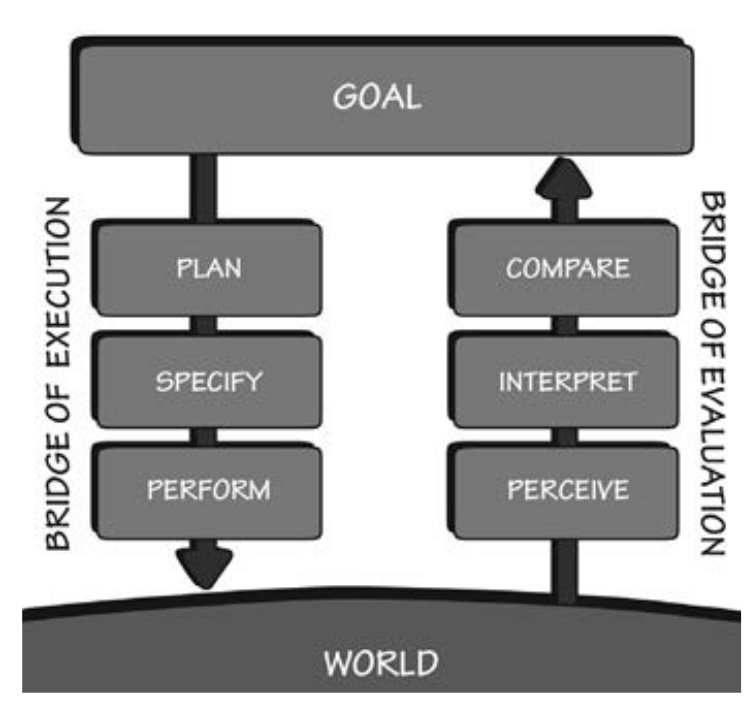
\includegraphics[width=0.5\textwidth]{figures/chapter1/Norman_7_stages_action.png}
\caption{The seven stages of actions defined by Norman \cite{norman2013design}. By giving a precise definition of each stage, this model guides the design and engineering of interactive systems by emphasizing each step of the cognitive processes taking place during an action. The designer can estimate the scope of the system and the potential errors at each stage of action.}
\label{fig:norman_7_stages}
\end{figure}

Indeed, too many systems require an expertise to be used. This often results from the system designer focusing on the ``machine part'' and not on the interface. Machines have been identified to avoid some humans flaws for a long time \cite{fitts_human_1951}, but because the ``interface'' \footnote{We refer here to the first meaning of ``interface'': the common surface where two systems meet and interact.} is too often poorly designed, the human needs to make great effort to use the machine. This effort becomes more important as the system gains in complexity and automation. This has been identified by Norman as the ``paradox of automation'' \cite{norman2013design}. More precisely, when an automation is performing a task the human situation awareness \cite{endsley_design_1988} decreases leading to misuses and errors when they need to interact with the system (\textit{e.g.} because of a system error or incapability).

\subsubsection{Human Robot Interaction}
When interacting with a robot, the human is no more the only agent taking autonomous decisions and able to act on the world. Indeed, not only the robot has its own plan-act-sense cycle with its own goal, but it can also physically move and change its environment. For the decision part, Bradshaw \textit{et al.} \cite{bradshaw2011human} propose eight maxims to complete and specify the recommendations of Norman. These maxims apply to human-agent interaction when they perform a joint activity:
\begin{itemize}
\item The agent must be \textit{observable}: its state and intentions are clearly exposed to others.
\item The agent must \textit{appraise progress}: it should inform others about the status of its task and warn them for any foreseen potential issues.
\item The agent must \textit{know its limits}: it should be proactive or wait when performing a task, depending on its evaluation of its capabilities.
\item The agent must be \textit{predictable} and \textit{dependable}: it should show what its capabilities are, and be trusted to use them at its best.
\item The agent must be \textit{directable}: its (sub)task can be preempted or modified if required and its knowledge can be updated thanks to other agents.
\item The agent must be \textit{selective}: it should expose only relevant facts in the context of the task.
\item The agent must be \textit{coordinated}: it should negotiate and deconflict plans, share resources and align beliefs between agents to create a \textit{common ground} if it is required to perform the task.
\end{itemize}

Interestingly, in their ``Architecture for autonomy'', Alami \textit{et al.} propose a robotic architecture which defines similar levels as the ones identified by Norman during human action \cite{alami1998architecture}.


% Focus on motion (navigation) => legibility, predictability, ...
Robot navigation should also respect these maxims. A number of approaches are trying to cope with these specific human robot issues \cite{kruse_human-aware_2013}. Moreover, more precise concepts have emerged from the maxims especially for the motion of a robot in a joint activity. 

First of all, the motion should ensure the physical safety of the surrounding humans. This is often respected by constraining the trajectory to stay at a minimal distance from humans \cite{kruse_human-aware_2013, rios2015proxemics}.

Moreover, while in a task, the motion of the robot can be used to convey information about its intentions, and thus making it more \textit{observable} and \textit{predictable}. Dragan \textit{et al.} defines three types of motions: functional, predictable and legible \cite{dragan2015effects}. A \textit{functional motion} is built only to make the robot move from on state to another one while avoiding humans and obstacles, it does not aim at providing any intent --- which does not mean it does not provide one. Then, a \textit{predictable motion} is a motion expected by an external observer knowing the robot model and its goal. It is often the quickest or shortest trajectory to reach the goal. Finally, a \textit{legible motion} is a motion allowing an external observer to quickly and reliably infer the robot motion goal.

However, as identified by Sisbot \textit{et al.}, to be identified as legible or predictable, the robot motion must be seen by the human. Accounting for the visibility of the robot by the human is paramount \cite{sisbot_human_2007}.  They integrate this constraint in a motion planner which is able to compute the safety of trajectories using the distance to a specified human and also prioritize visibility of the robot by estimating the field of view of the human and penalizing trajectories outside of it.

A lot of work has been made to generate legible paths. In \cite{beetz2010generality}, the robot learns usual motions from humans and generates trajectories based on them. However, even if the authors highlights the improvement in legibility, one could argue that the learned motions correspond more to the Dragan's definition of \textit{predictability}. In \cite{dragan_legibility_2013}, a robot motion planner is presented which is dedicated to generate legible trajectory. They prove its effectiveness through a user study while reporting an interesting finding: if the legibility of the motion is stressed to much, it becomes unpredictable and confuses the observer.




\subsection{Joint Action in Human-Robot Interaction}

Besides designing behaviors from scratch, previous work takes inspiration from situations where humans already perform a task with another autonomous agent: another human. Several previous contributions have been done studying how humans perform a so-called \textit{joint action}. \textit{Joint action} is defined by Sebanz \textit{et al.} as ``any form of social interaction whereby two or more individuals coordinate their actions in space and time to bring about a change in the environment'' \cite{sebanz2006joint}. Moreover, several work investigate multiple key abilities humans deploy when performing a joint action:
\begin{itemize}
\item humans can create and understand \textit{joint attention}: they are able to direct, or be directed by, others' attention \cite{pacherie_phenomenology_2011, sebanz2006joint}.
\item humans can \textit{predict} others' action effects and goals \cite{tomasello2005understanding, sebanz2006joint}.
\item humans can \textit{represent the shared task}: they can infer others' actions without directly seeing it, by observing events in the environment \cite{knoblich2011psychological, sebanz2006joint}.
\item humans can \textit{coordinate actions} by integrating others' actions into their own plan \cite{sebanz2006joint}.
\item humans consider combined actions results more important than their own only \cite{sebanz2006joint}.
\item yet, humans are able to \textit{distinguish their own actions from other's}, allowing them to find any divergence in beliefs or intentions and align them (\textit{e.g. through communication} if necessary \cite{pacherie_phenomenology_2011}.
\end{itemize}

Besides, a joint action can only occur if the involved agents know the presence of others agents but also their activity and intentions. Pacherie defines it as the mutual manifestness: ``\textit{each subject must be aware, in some sense, of the event as an event that is present to both; in other words the fact that both are attending to the same object or event should be open or mutually manifest}'' \cite{pacherie_phenomenology_2011}. Thus, it is not only necessary for the agents to account for the presence of the other but they also need to know they are involved in the same task.

Finally, studies show that humans can help the others to predict and coordinate their actions by communicating or slightly modifying their own. Coordination smoothers are defined as the changes in an agent own behavior to ease the interaction with another one \cite{vesper_minimal_2010}.

It is interesting to note that some concepts are already overlapping with the desirable features for a robot taking part in an activity with a human. For example, the legibility and predictability of motion are based on models of the human capability to understand coordination smoothers and predict future actions effects. Bradshaw \textit{et al.} also refer to an ``extra work'' an agent has to perform to ensure an efficient interaction with a human partner \cite{bradshaw2003adjustable}, which can be linked to the mutual manifestness and the several mechanisms which can be used, and which a human expects, when interacting.

Moreover, some work already try to incorporate these joint action concepts and abilities into robotic architectures and behaviors \cite{khamassi2016integration, clodic2017key}. Lemaignan et al. present a robotic architecture composed of several components addressing the cognitive skills required to perform a collaborative task \cite{lemaignan2017artificial}. These include shared plan synthesis, human-aware motion planning --- both of which discussed later in this chapter ---, supervision, beliefs management and situation assessment. The situation assessment is able to generate symbolic facts from geometric data for the robot and also to estimate the beliefs of the human partner based on an estimation of their perspective of the scene \cite{milliez2014framework}. This framework has since been improved to a more modular approach allowing more refined reasoning, especially for the estimation of human beliefs \cite{lemaignan2018underworlds}. The supervision component is based on SHARY \cite{clodic2009shary} allowing the robot to execute shared plan while monitoring the human activities and deciding when to communicate. Devin \& Alami proposed an extended supervision system, heavily based on theory of mind, which is able to follow a shared plan but also to compute diverging agents beliefs, deciding if the divergence endangers the plan and if so, align the beliefs via verbal communications \cite{devin2016implemented}.

\section{Modeling Human Actions and Shared Plans}

It has been shown previously that a robotic agent interacting with a human needs to coordinate its actions with them. Moreover, joint action theory exhibits that humans interacting together are able to represent the task as a whole, and plan not only for their actions but also for the actions of other agents. Thus, we think that for a human to perform the most efficient and satisfactory joint task with a robot, this robot must explicitly model the human actions and plan not only for its actions but also for the human ones. In this part we will first introduce some notations used throughout all this thesis, then we will briefly show some ways of modeling human task and link them with robot task planning. Finally, we review some systems planning for both humans and robots when performing a joint task.

\subsection{Notations}
In order to help to differentiate between the models presented in this thesis, we introduce here some notations we will use in the thesis. These notations are partially inspired by from the work of Chakraborti \textit{et al.} \cite{chakraborti2018human}. We will refer to the model the robot has of itself as $\robotmodel$, to the model the robot has of the human it is interacting with as $\humanmodel$ and to the model the human has of the robot as $\robotinhumanmodel$. The models can represent different parts of the agent, ranging from their beliefs to their action model, while not being here a formal definition, the notation should help to understand to which agent we are referring to. It is important to note that all the components presented in this thesis are considered to be a part of the robot, and thus $\robotmodel$ plays a special role as we consider all the information in it as the ground truth. For example, if there is a belief divergence between $\robotmodel$ and $\humanmodel$, we always consider that the $\robotmodel$ is the truth, otherwise, it would make no sense to keep this information in $\robotmodel$ while having access to the one in $\humanmodel$.

\begin{figure}
\centering
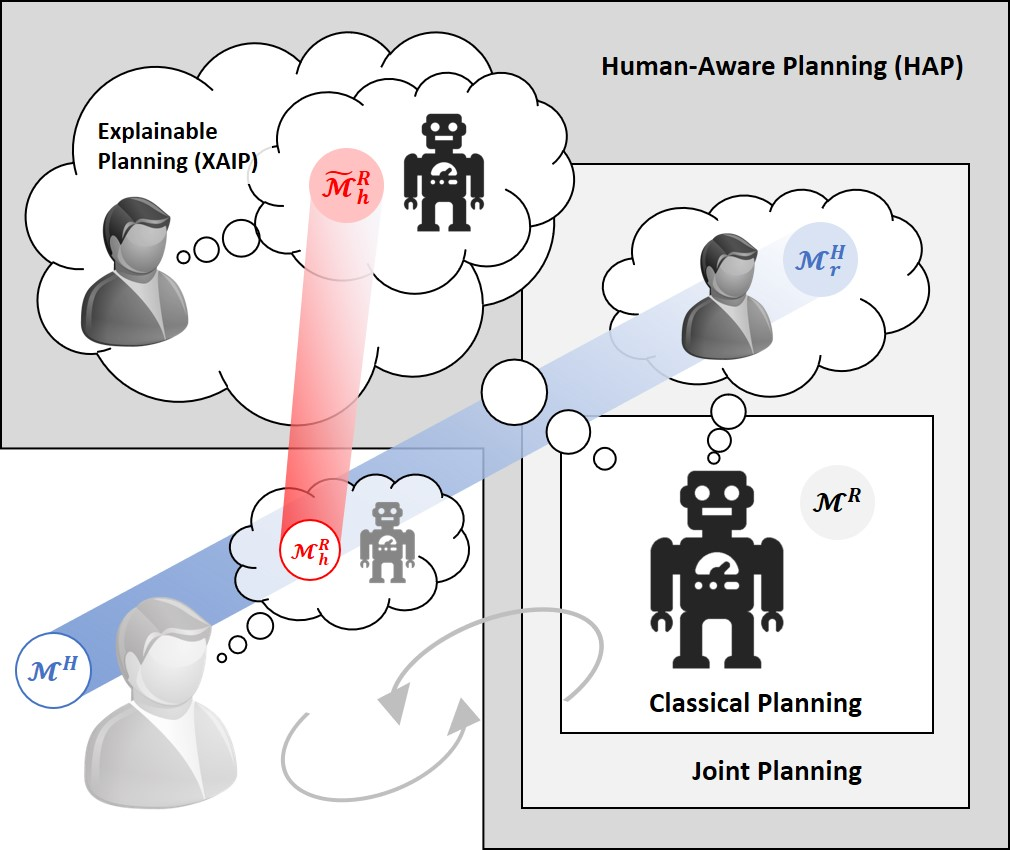
\includegraphics[width=0.7\textwidth]{figures/chapter1/chkraborti3models.png}
\caption{The notation coined by Chakraborti \textit{et al.} from \cite{chakraborti2018human} to represent the robot model $\robotmodel$, the estimated human model $\humanmodel$ and the estimated robot model the human has $\tilde{\robotinhumanmodel}$ (denoted $\robotinhumanmodel$ for simplicity as the real one is not accessible to the robot).}
\label{fig:chakraborti3models}
\end{figure}

\subsection{Task Modeling and Hierarchical Task Networks}
%, Hamster, Nau
Multiple approaches try to model the human activity. It is useful either for psychological studies, or to design a system that integrates gracefully in human tasks, in order to improve their performances. These tasks can be seen as hierarchical, where abstract ones decompose into smaller, more concrete ones. Such a hierarchical approach is also used in order to elaborate plans for autonomous robots. Interestingly the underlying structures share several commonalities.

\subsubsection{Human Task Modeling}
A common way of representing human activity ($\humanmodel$) and interaction with computer at high abstraction level is by using \textit{task models}. The hierarchical structure of human activity was first exploited by Annett and Duncan \cite{annett1967task}. They state that tasks can be described at several levels of abstraction until a certain criterion is met. Each task can thus be refined into subtasks detailing the procedure followed by the human to achieve the higher level task.
Task modeling has then evolved to introduce interaction with systems, produced and needed information, potential errors and a wide variety of operators specifying how tasks interacts with each other during their execution. Task models are now commonly used in user-centered and user interface designing processes. Most advanced notations include \textit{ConcurTaskTrees} \cite{paterno2004concurtasktrees} and \textit{HAMSTERS} \cite{martinie2019analysing}.
These models are used to design or to evaluate interactive systems. It allows the designer to better understand the user task or to study the user workflow using their system. However, these models contains to little information for a system to be able to reason and take decision on them (either in planning or acting).

\subsubsection{Robot Hierarchical Task Planning}
On the other hand, hierarchical representation of tasks are also used for decades in robotic planning ($\robotmodel$). In classical planning, each action of an agent is atomic and need some conditions to hold in the environment to be executed, then it changes the environment when applied. The planning process has then to find the right sequence of actions, being applicable one after the other to change the environment to reach a certain goal state. \acrfullpl{htn} allow the domain designer to help the plan search by inserting a hierarchy between these actions \cite{erol1996complexity}. Indeed, a network is composed of one or several tasks or actions, and each task has one or several decompositions. Each decomposition is itself a task network. The goal of the planner is not to find the sequence of actions to reach a goal, but rather to select recursively for each task the right decomposition ending (if possible) with a network of actions applicable from the initial state. Such a process is named by Ghallab, Nau and Traverso as \textit{planning with refinement methods} \cite{ghallab_nau_traverso_2016}.

This planning hierarchy not only allows the domain designer to guide the search by inserting some expertise into the model, but also to enhance explainability as the decompositions often offers a semantic to the subtask (the \textit{why} can usually be answered by going up in the hierarchy, while the \textit{how} is answered by going down).
% However used for evaluating or designing systems, but the system do not take decision based on it.
% Similar (hierarcical) HTN for robot planning... 

\subsection{Planning for Both the Human and the Robot}
%Charkrabori, Shah, HATP Jules, Epistemic planning?
While human activity modeling and autonomous planning have been studied separately for decades, there are still only few systems proposing to incorporate human activity into planning for intricate interactive tasks.
Planning for both a robotic agent and a human is not trivial. Indeed, while the robotic agent is planning for itself and will surely execute the plan, the human is not directly controllable (making them follow the plan may require the robot to at least communicate and perhaps negotiate) and can also has a plan themselves they are trying to execute.

The \acrfull{hatp} proposes a hierarchical approach to multi agent task planning \cite{alili2009task, lallement2014hatp}. This \acrshort{htn} based planner is able to elaborate a multi agent plan based on a single \acrshort{htn} tree (unifying both $\robotmodel$ and $\humanmodel$). Moreover, it maintains one belief base per agent allowing to write task decomposition rules and actions preconditions and effects in any agent belief base. Finally, \acrshort{hatp} also computes costs for the found plans based on action costs and predefined social rules. More details about HATP will be presented in Chapter~\ref{chapter:comm}. This task planner has been coupled with the Geometrical Task Planner (GTP) allowing to also plan the geometrical motion of the human partner to inform HATP about the feasibility and the cost of a motion action \cite{gharbi2015combining}. As stated before, HATP has been used in complete robotic architecture \cite{devin2016implemented, lemaignan2017artificial}.

Buckingham \textit{et al.} propose a planning scheme questioning humans mental models ($\humanmodel$) returning the effects of expected future humans actions \cite{buckingham2020robot}. The planner is then able to determine a robot policy ($\robotmodel$) influencing the humans actions. In this work, they show how this framework is able to cope with interactive tasks even without assuming that the human is collaborating.

Similarly, Unhelkar \textit{et al.} proposed a POMDP-based approach called CommPlan \cite{unhelkar2020decision}. The POMDP is built using a user defined MDP (Markov Decision Process) representing the collaborative task and an AMM (Agent Markov Model) to represent the human decision-making process ($\humanmodel$). This POMDP is then solved to produce a robot policy ($\robotmodel$) which, in particular, decides when the robot has to communicate about its beliefs, to question the human about theirs and to ask the human to perform an action. Besides, the human AMM ($\humanmodel$) is not only specified by the programmer but also refined during the interaction via learning.

Besides, to cope with the uncertainty of the human knowledge ($\humanmodel$), Petrick and Foster propose to use conditional planning allowing to plan for incomplete information~\cite{petrick2013planning}. By doing so, the planner elaborates a plan for the robot ($\robotmodel$) accounting for multiple possible human choices, and depending on the knowledge received the execution component can execute the right branch of the plan.

Likewise, Sanelli \textit{et al.} (\cite{sanelli2017short}) present an approach not only elaborating conditional plans for the robot ($\robotmodel$)  depending on the possible human choices ($\humanmodel$, \textit{e.g.} the choice of activity the human wants to perform), but they are able to transform this conditional plan into a Petri net plan to handle its execution. This contribution is inspired from a previous work by Nardi and Iocchi (\cite{nardi2014representation}) in which they present a method for transforming (linear) joint plan (both $\robotmodel$ and $\humanmodel$) into a Petri net plan managing its execution. Interestingly, the human actions from the plan are changed into a part of the Petri net where the robot elicit the action (\textit{e.g.} via a verbal communication) if the human does not perform it by themselves. However, this approach only request the human to make single actions, instead of sharing a high level goal, which can become unpleasant if done repeatedly. 

Chakraborti \textit{et al.} uses both the robot model ($\robotmodel$) and the estimation of the model the human has of the robot ($\robotinhumanmodel$) to improve plan explicability \cite{chakraborti2017plan}. Indeed, they propose a novel approach called model reconciliation which they present as a classical planning problem. In this problem, the goal is to make identical the both optimal plans generated via the robot model $\robotmodel$ and the human estimation of the robot model $\robotinhumanmodel$. To do so, they define a list of operators on the models in order to modify them until the plans matches. To our knowledge it is the only approach both reasoning on $\robotinhumanmodel$ and operating directly on the action models. However, it only has been applied to robot plans and not to joint plans. Indeed, the plans generated contain robot actions only, and the robot and the human do not directly collaborate in the presented tasks.

% Geometrical collabortaive planning (HATEB, Jules)
Geometrical planning in human robot activity has also been studied in several works. For navigation, Khambhaita and Alami proposed a planner which optimizes both the human and the robot trajectories ($\robotmodel$ and $\humanmodel$) \cite{khambhaita_viewing_2017}. This allows the robot not only to have a prediction of the human future trajectory, but also to model their interactions and how its own trajectory can affect the human's one. The approach will be detailed in Chapter~\ref{chapter:navigation}.

Besides, representing humans as a group has also been showed as beneficial for robot navigation. For instance, for the robot-waiters problem, where multiple robots compute trajectories in order to serve multiple moving humans in a room containing obstacles, Saraydaryan \textit{et al.} (\cite{saraydaryan2015robots}) showed that considering clusters of humans to be served allows to decrease the human idleness (the duration for which a human has not been served by a robot). These humans clusters are called F-Formations when the human are actively interacting with each other in the cluster (\textit{e.g.} a group of human discussing together). Recognizing them and integrating them ($\humanmodel$) in the robot trajectory computation ($\robotmodel$) in order to socially integrate them or to not disturb them also allows for more acceptable robot trajectories (\cite{althaus2004navigation}).

Another work presents a motion planner allowing to balance the effort between the robot and the human, depending on the mobility of the human, for a handover task \cite{mainprice2012sharing}. To do so, they sample an acceptable position for the human ($\humanmodel$) according to several parameters, including its settable mobility, then they try to plan a trajectory for both the robot ($\robotmodel$) and the human ($\humanmodel$) to get them into an handover configuration. This work has then be extended and generalized by Waldhart, Gharbi and Alami to handle several robots and humans \cite{waldhart2015planning}.

Finally, Waldhart, Clodic and Alami proposed a geometric planner, able to find the best robot and human positions for the robot to point a landmark at the human \cite{waldhart_reasoning_shared_2019}. This planner uses the human vision ability and mobility ($\humanmodel$) as well as robot mobility and respect of a pointing triangle formation between the robot, the human and the landmark to point ($\robotmodel$).

From all these contributions we see a great interest in planning for both the human and the robot. Indeed, they allow to represent multiple features highly desired in human robot interaction scenarios. First, by planning for both, shared goals and coordinated actions can be represented. The planners are able to elaborate plans (or trajectories) that do not conflict between the agents, and even that interact in a collaborative way to reach the shared goal. 

Then, it allows to attribute tasks to either one agent or the other if they can be done by both. Unlike other task attribution approaches, modeling the human helps to estimate the effort taken in the contribution of the joint plan. The planner can ensure that most of the effort is taken by the robot but can also balance other solutions depending on the context (\textit{e.g.} urgency to perform the task, where the human may accept to contribute more to do it faster). 

Finally, when integrated in a robotic architecture and in a real human robot scenario, planning for both reveals to be key. Indeed, planning before acting usually avoids deadlocks during execution or sub-optimal solutions which would have been encountered by only reasoning on short term. But for human robot interaction it also allows to estimate the effort and the contribution of each agent \textit{before involving the human}. Moreover, the resulting joint plan can then be negotiated with the human before starting the task, allowing for a better efficiency, satisfaction, explainability and acceptability.

Not all of these challenges have been entirely tackled yet. In this thesis we propose to explore multiple ways of planning for both agents. 

\ifdefined\included
\else
\bibliographystyle{acm}
\bibliography{These}
\end{document}
\fi

